
%% bare_conf.tex
%% V1.4b
%% 2015/08/26
%% by Michael Shell
%% See:
%% http://www.michaelshell.org/
%% for current contact information.
%%
%% This is a skeleton file demonstrating the use of IEEEtran.cls
%% (requires IEEEtran.cls version 1.8b or later) with an IEEE
%% conference paper.
%%
%% Support sites:
%% http://www.michaelshell.org/tex/ieeetran/
%% http://www.ctan.org/pkg/ieeetran
%% and
%% http://www.ieee.org/

%%*************************************************************************
%% Legal Notice:
%% This code is offered as-is without any warranty either expressed or
%% implied; without even the implied warranty of MERCHANTABILITY or
%% FITNESS FOR A PARTICULAR PURPOSE! 
%% User assumes all risk.
%% In no event shall the IEEE or any contributor to this code be liable for
%% any damages or losses, including, but not limited to, incidental,
%% consequential, or any other damages, resulting from the use or misuse
%% of any information contained here.
%%
%% All comments are the opinions of their respective authors and are not
%% necessarily endorsed by the IEEE.
%%
%% This work is distributed under the LaTeX Project Public License (LPPL)
%% ( http://www.latex-project.org/ ) version 1.3, and may be freely used,
%% distributed and modified. A copy of the LPPL, version 1.3, is included
%% in the base LaTeX documentation of all distributions of LaTeX released
%% 2003/12/01 or later.
%% Retain all contribution notices and credits.
%% ** Modified files should be clearly indicated as such, including  **
%% ** renaming them and changing author support contact information. **
%%*************************************************************************


% *** Authors should verify (and, if needed, correct) their LaTeX system  ***
% *** with the testflow diagnostic prior to trusting their LaTeX platform ***
% *** with production work. The IEEE's font choices and paper sizes can   ***
% *** trigger bugs that do not appear when using other class files.       ***                          ***
% The testflow support page is at:
% http://www.michaelshell.org/tex/testflow/


\documentclass[conference]{IEEEtran}
% Some Computer Society conferences also require the compsoc mode option,
% but others use the standard conference format.
%
% If IEEEtran.cls has not been installed into the LaTeX system files,
% manually specify the path to it like:
% \documentclass[conference]{../sty/IEEEtran}
%\documentclass{ifacconf}




% Some very useful LaTeX packages include:
% (uncomment the ones you want to load)


% *** MISC UTILITY PACKAGES ***
%
%\usepackage{ifpdf}
% Heiko Oberdiek's ifpdf.sty is very useful if you need conditional
% compilation based on whether the output is pdf or dvi.
% usage:
% \ifpdf
%   % pdf code
% \else
%   % dvi code
% \fi
% The latest version of ifpdf.sty can be obtained from:
% http://www.ctan.org/pkg/ifpdf
% Also, note that IEEEtran.cls V1.7 and later provides a builtin
% \ifCLASSINFOpdf conditional that works the same way.
% When switching from latex to pdflatex and vice-versa, the compiler may
% have to be run twice to clear warning/error messages.






% *** CITATION PACKAGES ***
%
%\usepackage{cite}
% cite.sty was written by Donald Arseneau
% V1.6 and later of IEEEtran pre-defines the format of the cite.sty package
% \cite{} output to follow that of the IEEE. Loading the cite package will
% result in citation numbers being automatically sorted and properly
% "compressed/ranged". e.g., [1], [9], [2], [7], [5], [6] without using
% cite.sty will become [1], [2], [5]--[7], [9] using cite.sty. cite.sty's
% \cite will automatically add leading space, if needed. Use cite.sty's
% noadjust option (cite.sty V3.8 and later) if you want to turn this off
% such as if a citation ever needs to be enclosed in parenthesis.
% cite.sty is already installed on most LaTeX systems. Be sure and use
% version 5.0 (2009-03-20) and later if using hyperref.sty.
% The latest version can be obtained at:
% http://www.ctan.org/pkg/cite
% The documentation is contained in the cite.sty file itself.






% *** GRAPHICS RELATED PACKAGES ***
%
%\ifCLASSINFOpdf
  % \usepackage[pdftex]{graphicx}
  % declare the path(s) where your graphic files are
  % \graphicspath{{../pdf/}{../jpeg/}}
  % and their extensions so you won't have to specify these with
  % every instance of \includegraphics
  % \DeclareGraphicsExtensions{.pdf,.jpeg,.png}
%\else
  % or other class option (dvipsone, dvipdf, if not using dvips). graphicx
  % will default to the driver specified in the system graphics.cfg if no
  % driver is specified.
  % \usepackage[dvips]{graphicx}
  % declare the path(s) where your graphic files are
  % \graphicspath{{../eps/}}
  % and their extensions so you won't have to specify these with
  % every instance of \includegraphics
  % \DeclareGraphicsExtensions{.eps}
%\fi
% graphicx was written by David Carlisle and Sebastian Rahtz. It is
% required if you want graphics, photos, etc. graphicx.sty is already
% installed on most LaTeX systems. The latest version and documentation
% can be obtained at: 
% http://www.ctan.org/pkg/graphicx
% Another good source of documentation is "Using Imported Graphics in
% LaTeX2e" by Keith Reckdahl which can be found at:
% http://www.ctan.org/pkg/epslatex
%
% latex, and pdflatex in dvi mode, support graphics in encapsulated
% postscript (.eps) format. pdflatex in pdf mode supports graphics
% in .pdf, .jpeg, .png and .mps (metapost) formats. Users should ensure
% that all non-photo figures use a vector format (.eps, .pdf, .mps) and
% not a bitmapped formats (.jpeg, .png). The IEEE frowns on bitmapped formats
% which can result in "jaggedy"/blurry rendering of lines and letters as
% well as large increases in file sizes.
%
% You can find documentation about the pdfTeX application at:
% http://www.tug.org/applications/pdftex





% *** MATH PACKAGES ***
%
%\usepackage{amsmath}
% A popular package from the American Mathematical Society that provides
% many useful and powerful commands for dealing with mathematics.
%
% Note that the amsmath package sets \interdisplaylinepenalty to 10000
% thus preventing page breaks from occurring within multiline equations. Use:
%\interdisplaylinepenalty=2500
% after loading amsmath to restore such page breaks as IEEEtran.cls normally
% does. amsmath.sty is already installed on most LaTeX systems. The latest
% version and documentation can be obtained at:
% http://www.ctan.org/pkg/amsmath





% *** SPECIALIZED LIST PACKAGES ***
%
%\usepackage{algorithmic}
% algorithmic.sty was written by Peter Williams and Rogerio Brito.
% This package provides an algorithmic environment fo describing algorithms.
% You can use the algorithmic environment in-text or within a figure
% environment to provide for a floating algorithm. Do NOT use the algorithm
% floating environment provided by algorithm.sty (by the same authors) or
% algorithm2e.sty (by Christophe Fiorio) as the IEEE does not use dedicated
% algorithm float types and packages that provide these will not provide
% correct IEEE style captions. The latest version and documentation of
% algorithmic.sty can be obtained at:
% http://www.ctan.org/pkg/algorithms
% Also of interest may be the (relatively newer and more customizable)
% algorithmicx.sty package by Szasz Janos:
% http://www.ctan.org/pkg/algorithmicx


%IEEE
\usepackage{graphicx}      % include this line if your document contains figures
%\usepackage{natbib}        % required for bibliography
\usepackage{float}
\usepackage{amssymb}
\usepackage{amsmath}
\newtheorem{theorem}{Theorem}
\newtheorem{proof}{Proof}

\usepackage{balance}

%IFAC
%\usepackage{graphicx}      % include this line if your document contains figures
%\usepackage{natbib}        % required for bibliography
%\usepackage{float}
%\usepackage{amssymb}
%\usepackage{amsmath}



% *** ALIGNMENT PACKAGES ***
%
%\usepackage{array}
% Frank Mittelbach's and David Carlisle's array.sty patches and improves
% the standard LaTeX2e array and tabular environments to provide better
% appearance and additional user controls. As the default LaTeX2e table
% generation code is lacking to the point of almost being broken with
% respect to the quality of the end results, all users are strongly
% advised to use an enhanced (at the very least that provided by array.sty)
% set of table tools. array.sty is already installed on most systems. The
% latest version and documentation can be obtained at:
% http://www.ctan.org/pkg/array


% IEEEtran contains the IEEEeqnarray family of commands that can be used to
% generate multiline equations as well as matrices, tables, etc., of high
% quality.




% *** SUBFIGURE PACKAGES ***
%\ifCLASSOPTIONcompsoc
%  \usepackage[caption=false,font=normalsize,labelfont=sf,textfont=sf]{subfig}
%\else
%  \usepackage[caption=false,font=footnotesize]{subfig}
%\fi
% subfig.sty, written by Steven Douglas Cochran, is the modern replacement
% for subfigure.sty, the latter of which is no longer maintained and is
% incompatible with some LaTeX packages including fixltx2e. However,
% subfig.sty requires and automatically loads Axel Sommerfeldt's caption.sty
% which will override IEEEtran.cls' handling of captions and this will result
% in non-IEEE style figure/table captions. To prevent this problem, be sure
% and invoke subfig.sty's "caption=false" package option (available since
% subfig.sty version 1.3, 2005/06/28) as this is will preserve IEEEtran.cls
% handling of captions.
% Note that the Computer Society format requires a larger sans serif font
% than the serif footnote size font used in traditional IEEE formatting
% and thus the need to invoke different subfig.sty package options depending
% on whether compsoc mode has been enabled.
%
% The latest version and documentation of subfig.sty can be obtained at:
% http://www.ctan.org/pkg/subfig




% *** FLOAT PACKAGES ***
%
%\usepackage{fixltx2e}
% fixltx2e, the successor to the earlier fix2col.sty, was written by
% Frank Mittelbach and David Carlisle. This package corrects a few problems
% in the LaTeX2e kernel, the most notable of which is that in current
% LaTeX2e releases, the ordering of single and double column floats is not
% guaranteed to be preserved. Thus, an unpatched LaTeX2e can allow a
% single column figure to be placed prior to an earlier double column
% figure.
% Be aware that LaTeX2e kernels dated 2015 and later have fixltx2e.sty's
% corrections already built into the system in which case a warning will
% be issued if an attempt is made to load fixltx2e.sty as it is no longer
% needed.
% The latest version and documentation can be found at:
% http://www.ctan.org/pkg/fixltx2e


%\usepackage{stfloats}
% stfloats.sty was written by Sigitas Tolusis. This package gives LaTeX2e
% the ability to do double column floats at the bottom of the page as well
% as the top. (e.g., "\begin{figure*}[!b]" is not normally possible in
% LaTeX2e). It also provides a command:
%\fnbelowfloat
% to enable the placement of footnotes below bottom floats (the standard
% LaTeX2e kernel puts them above bottom floats). This is an invasive package
% which rewrites many portions of the LaTeX2e float routines. It may not work
% with other packages that modify the LaTeX2e float routines. The latest
% version and documentation can be obtained at:
% http://www.ctan.org/pkg/stfloats
% Do not use the stfloats baselinefloat ability as the IEEE does not allow
% \baselineskip to stretch. Authors submitting work to the IEEE should note
% that the IEEE rarely uses double column equations and that authors should try
% to avoid such use. Do not be tempted to use the cuted.sty or midfloat.sty
% packages (also by Sigitas Tolusis) as the IEEE does not format its papers in
% such ways.
% Do not attempt to use stfloats with fixltx2e as they are incompatible.
% Instead, use Morten Hogholm'a dblfloatfix which combines the features
% of both fixltx2e and stfloats:
%
% \usepackage{dblfloatfix}
% The latest version can be found at:
% http://www.ctan.org/pkg/dblfloatfix




% *** PDF, URL AND HYPERLINK PACKAGES ***
%
%\usepackage{url}
% url.sty was written by Donald Arseneau. It provides better support for
% handling and breaking URLs. url.sty is already installed on most LaTeX
% systems. The latest version and documentation can be obtained at:
% http://www.ctan.org/pkg/url
% Basically, \url{my_url_here}.




% *** Do not adjust lengths that control margins, column widths, etc. ***
% *** Do not use packages that alter fonts (such as pslatex).         ***
% There should be no need to do such things with IEEEtran.cls V1.6 and later.
% (Unless specifically asked to do so by the journal or conference you plan
% to submit to, of course. )


% correct bad hyphenation here
%\hyphenation{op-tical net-works semi-conduc-tor}


\begin{document}
%\begin{frontmatter}
%
% paper title
% Titles are generally capitalized except for words such as a, an, and, as,
% at, but, by, for, in, nor, of, on, or, the, to and up, which are usually
% not capitalized unless they are the first or last word of the title.
% Linebreaks \\ can be used within to get better formatting as desired.
% Do not put math or special symbols in the title.
\title{Architecture for Testing Learning-Based Autonomous Vehicle Control Design}

% author names and affiliations
% use a multiple column layout for up to three different
% affiliations

%IEEE
\author{
\IEEEauthorblockN{Michael Kogan}
\IEEEauthorblockA{Department of Electrical and\\Computer Engineering\\
Royal Military College of Canada\\
Kingston, Ontario, Canada\\
Email: Michael.Kogan@forces.gc.ca}
\and
\IEEEauthorblockN{Peter T. Jardine}
\IEEEauthorblockA{Department of Electrical and\\Computer Engineering\\
Royal Military College of Canada\\
Kingston, Ontario, Canada\\
Email:  peter.jardine@rmc.ca}
\and
\IEEEauthorblockN{Sidney N. Givigi}
\IEEEauthorblockA{Department of Electrical and\\Computer Engineering\\
Royal Military College of Canada\\
Kingston, Ontario, Canada\\
Email: sidney.givigi@rmc.ca}}





%IFAC
%\author[First]{Peter T. Jardine} 
%\author[First]{Sidney Givigi} 
%\author[Third]{Shahram Yousefi}
%
%\address[First]{Department of Electrical and Computer Engineering, Royal Military College of Canada, Kingston,
%Ontario, Canada (e-mail: peter.jardine@rmc.ca, sidney.givigi@rmc.ca)}
%%\address[Second]{Department of Electrical and Computer Engineering, Royal Military College of Canada, Kingston,
%%Ontario, Canada (e-mail: sidney.givigi@rmc.ca)}
%\address[Third]{Department of Electrical and Computer Engineering, Queen's University, Kingston,
%Ontario, Canada (e-mail: s.yousefi@queensu.ca)}

% conference papers do not typically use \thanks and this command
% is locked out in conference mode. If really needed, such as for
% the acknowledgment of grants, issue a \IEEEoverridecommandlockouts
% after \documentclass

% for over three affiliations, or if they all won't fit within the width
% of the page, use this alternative format:
% 
%\author{\IEEEauthorblockN{Michael Shell\IEEEauthorrefmark{1},
%Homer Simpson\IEEEauthorrefmark{2},
%James Kirk\IEEEauthorrefmark{3}, 
%Montgomery Scott\IEEEauthorrefmark{3} and
%Eldon Tyrell\IEEEauthorrefmark{4}}
%\IEEEauthorblockA{\IEEEauthorrefmark{1}School of Electrical and Computer Engineering\\
%Georgia Institute of Technology,
%Atlanta, Georgia 30332--0250\\ Email: see http://www.michaelshell.org/contact.html}
%\IEEEauthorblockA{\IEEEauthorrefmark{2}Twentieth Century Fox, Springfield, USA\\
%Email: homer@thesimpsons.com}
%\IEEEauthorblockA{\IEEEauthorrefmark{3}Starfleet Academy, San Francisco, California 96678-2391\\
%Telephone: (800) 555--1212, Fax: (888) 555--1212}
%\IEEEauthorblockA{\IEEEauthorrefmark{4}Tyrell Inc., 123 Replicant Street, Los Angeles, California 90210--4321}}




% use for special paper notices
%\IEEEspecialpapernotice{(Invited Paper)}




% make the title area
\maketitle

% As a general rule, do not put math, special symbols or citations
% in the abstract
\begin{abstract}
This paper presents the architecture for the testing of autonomous vehicle controllers designed using machine learning. A localization system feeds measurement data into a ground station. The ground station processes this data and provides the position of the vehicle to the controller, which has been tuned offline via machine learning. Control inputs are then generated and provided to the vehicle in order to accomplish the desired mission. The performance of the learned controller is compared to a nominal case. During the offline tuning process, a vehicle model is used to simulate the actual vehicle. Once tuning is complete, the parameters are used to control a real vehicle in order to accomplish the desired mission. The proposed architecture was tested by tuning a model predictive controller to guide a differential drive robot to a series of waypoints using a Reinforced Learning technique known as Learning Automata. The controller was then tested online with a similar but different problem on a real differential drive robot. The results showed that after tuning, the vehicle performed significantly better. This demonstrated that offline learning techniques can be used to optimally select controller parameters. 
\end{abstract}

% no keywords
%\begin{keyword}
%Model Predictive Control, Quadcopter, Reinforcement Learning
%\end{keyword}

%\end{frontmatter}


% For peer review papers, you can put extra information on the cover
% page as needed:
% \ifCLASSOPTIONpeerreview
% \begin{center} \bfseries EDICS Category: 3-BBND \end{center}
% \fi
%
% For peerreview papers, this IEEEtran command inserts a page break and
% creates the second title. It will be ignored for other modes.
%\IEEEpeerreviewmaketitle

\section{Introduction}
\label{cha:intro}

Architectures present a streamlined approach to solving a problem, and therefore exist for many different applications. One notable field where different architectures are used is in software engineering~\cite{8216936}. Another prominent use of architecture arises in the field of robotics, where different architectures exist for the design of robot behaviour~\cite{Murphy:2000}. The purpose of developing a testing architecture is to streamline the testing of new ideas so that the tests are fast and results are easily comparable. An architecture allows a designer to run the same tests in a controlled environment for each of his or her designs. This ensures that the test results are a good measure of performance, leading to the best design being chosen. The primary goal of an architecture is to be as modular as possible while still providing enough detail to streamline the process, in order to allow for a broad number of use cases.

This paper presents the architecture that was developed at the Royal Military College of Canada in order to test vehicles whose controllers have been designed using machine learning. The architecture involves a localization system, a ground station, a controller, a vehicle, and a learning environment. The model of the vehicle is used to simulate the vehicle's behaviour so that the controller can be tuned offline in a realistic environment. The tuned controller is then used to control the real vehicle. The localization system provides measurement data to the ground station, which provides accurate position and orientation feedback to the controller in real-time. The controller sends commands to the vehicle to ensure that it completes the mission. These commands are equivalent to the inputs that we would pass to the vehicle according to the vehicle model. Low level controllers on the robot are used to actuate the vehicle in accordance with these commands. 

The use of machine learning techniques to tune controllers is a relatively recent innovation in control engineering. Classically, controllers are tuned via trial-and-error~\cite{Suicmez-2014} and experience by taking into account the dynamics of the control problem~\cite{Camacho:1999}. More recent studies have proposed auto-tuning approaches based on particle swarm optimization~\cite{han:2006,suzuki:2007} and genetic algorithms~\cite{vanderlee:2008}. A Reinforcement Learning (RL) technique known as Learning Automata (LA) has been shown to be an effective way to tune the gains of a Proportional-Integral-Derivative (PID) controller~\cite{Barros-2015}. Recently, this learning technique has been applied to linear~\cite{JardineSys-2017,jardine:2017:IFAC} and non-linear Model Predictive Control (MPC)~\cite{cabral:2017}. 

With machine learning quickly becoming a heavily-researched topic in controller design, a testing architecture is required to provide a way for fast and effective comparison between different controllers. This architecture needs to be general enough to handle a variety of learning techniques, controllers, and vehicles. Additionally, a demonstration using a specific learning technique, controller, and vehicle needs to be performed to prove the efficacy of the testing architecture. 

In order to demonstrate the effectiveness of the testing architecture, an MPC was designed using LA to train a differential drive robot to follow a series of waypoints. LA was chosen as the training method because it has been demonstrated in the past that this technique works well for vehicle control tuning~\cite{Barros-2015,JardineSys-2017,jardine:2017:IFAC,cabral:2017}. A differential drive robot was used because it is a commonly used platform in robotics research. Lastly, MPC was chosen because it is currently at the forefront of controls research, being an advanced control technique that can make efficient use of energy resources while considering constraints~\cite{Mooryong:2014,Zhao:2015,Ramana-2016}. It was important to demonstrate that the architecture can handle a controller which is actively being researched. A real differential drive robot was then given a moving target to track in a real environment, and the performance was compared with a nominal case.

The remainder of this paper is organized as follows: Sections \ref{sec:Notation} describes the notation used throughout the paper; Section \ref{sec:Architecture} describes the system architecture; Section \ref{sec:VehicleModel} develops the vehicle model; Section \ref{sec:MPCForm} addresses the control aspect of this architecture; Section \ref{RLFA} presents machine learning with a focus on reinforcement learning; Section \ref{sec:SimulLearn} describes our implementation of the architecture; Section \ref{sec:Results} presents the results; and Section \ref{sec:conc} concludes the paper.

\section{Notation} \label{sec:Notation}

In this paper, scalars are represented by lowercase letters from the Greek and Latin alphabets. The dot notation ($\dot{x}$) is used for derivatives with respect to time. Vectors are written in bold lowercase font ($\mathbf{x}$), and matrices are represented by uppercase Latin letters ($A$). Sets are represented by uppercase symbols written in calligraphy mode ($\mathcal{A}$), and uppercase Greek letters ($\Gamma$) represent tuples. Bold uppercase Greek letters ($\mathbf{\Gamma}$) represent groups of tuples. Subscripts ($a_{i}$) are used to denote individual elements in a vector, or when applied to matrices denote matrices in a series. Superscripts ($\Gamma^{i}$) are used to represent an element in a tuple that corresponds to the superscript.

\section{System Architecture} \label{sec:Architecture}

This section describes the proposed system architecture. The architecture consists of a localization system, a ground station, a controller, a vehicle, and a learning environment. The vehicle itself consists of a vehicle computer taking command inputs and turning them into low level control signals, as well as actuators reacting to the low level control signals. The controller is tuned using a vehicle model to simulate the actual vehicle in the learning environment. In a simulator, the vehicle model and the controller can run much faster than real time, making offline learning substantially faster than online learning. Once the parameters have been determined, they are used to design the actual controller. The controller feeds control commands to the robot and receives feedback on the position of the robot via the localization system. The system can be seen in Fig. \ref{fig:Arch}.

\begin{figure}[tb]
\centering
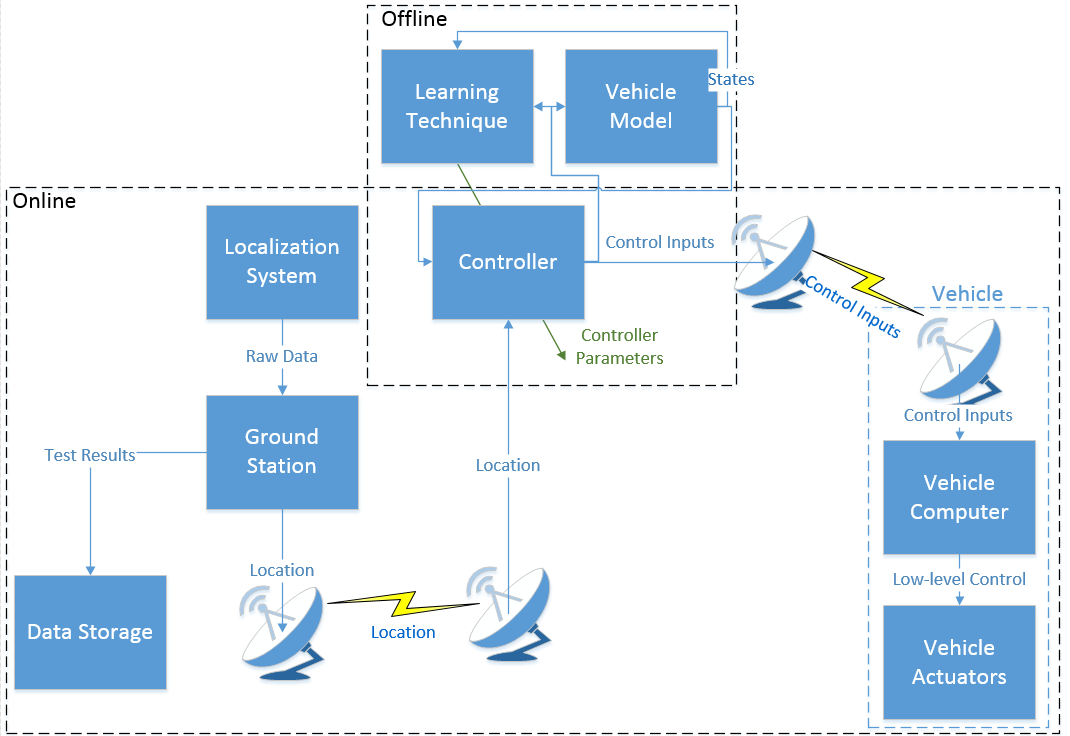
\includegraphics[width=80mm]{Arch.PNG}
\caption{Illustration of System Architecture for Vehicle Controller Testing}
\label{fig:Arch}
\end{figure} 

The localization system feeds measurement data to the ground station. The ground station is responsible for processing this data and sending the position and orientation data to the controller. The ground station is also responsible for saving relevant test data so that it may be compared with other results and used to validate the controller. The controller is tuned offline in the learning environment using a machine learning technique. The learning environment uses a model to simulate the vehicle during offline learning. Once the controller is tuned, it is brought online to control the vehicle. The learning environment itself is therefore not part of the online architecture, but rather a subsystem that tunes the controller prior to it coming online. The controller then generates control commands based on the position of the vehicle, the mission, and the parameters. These commands are sent to the vehicle wirelessly, in order to simulate a real-world environment where the controller and the vehicle could be running on different nodes of the network. The vehicle computer processes these commands and transforms them into low level control signals for the actuators of the vehicle.

The architecture presented is suitable for use with most common controllers, learning techniques, and vehicles. For the purposes of our experiment, we used the Optitrack localization system to provide data to the ground station, which used QUARC software to provide accurate position feedback to the controller. The controller was an MPC tuned with an RL technique known as LA. The vehicle was a differential drive robot, a Turtlebot running the Robot Operation System (ROS). ROS provided the functionality of the vehicle computer, taking commands and turning them into low level control signals for the Turtlebot's actuators.

\section{Vehicle Modeling} \label{sec:VehicleModel}

A vehicle model is required for the controller tuning process. We can define the movement of any vehicle using the following equation: $\mathbf{\dot{x}} = \mathbf{f(x, u)}$. This equation states that the change in the states of a vehicle is always a function of its current states $\mathbf{x}$ and the control inputs $\mathbf{u}$. 

\subsection{Overview}
The equation above is the most general description of an undisturbed vehicle with states dependent on previous states and inputs. The vehicle's model is used in the learning environment to simulate the behaviour of the vehicle. 

\subsection{Differential Drive Robot}
Let us now explore a specific example to see how the general vehicle equation can be applied. The kinematics of a differential drive robot can be described in terms of three states: position in Cartesian coordinates ($x$, $y$) and orientation $\theta$. The evolution of these states is controlled by two inputs, linear velocity $v$ and angular velocity $\omega$. The change of the orientation of the robot will depend solely on the angular velocity, and the change in $x$ and $y$ position will be a function of the linear velocity and the current orientation. To get the change in position in each axis, we project the velocity $v$ unto the $x$ and $y$ axes. This leads to the kinematics model for the differential drive robot~\cite{Siegwart:2004}:
$$
\begin{bmatrix}
\dot{x} \\
\dot{y} \\
\dot{\theta}
\end{bmatrix}
=
\begin{bmatrix}
v\cos(\theta) \\
v\sin(\theta) \\
\omega
\end{bmatrix}
$$

\section{Vehicle Control} \label{sec:MPCForm}

A controller is any system that generates signals to a plant in order to achieve the desired plant behaviour. A controller can also be subjected to a set of constraints in order to reflect the real world considerations of the system. The states of the system are observed via some sort of sensor, and then fed back to the controller in order to make the next control decision. 

\subsection{Overview}
In case of the presented architecture, the controller can be any controller with a feedback loop and the plant can be any vehicle. The sensor is a localization system, which provides position and orientation data about the vehicle. If other states are required, an observer can be used to estimate them. The key difference between this architecture and typical controllers is that here the parameters of the controller may be modified offline through a learning process, which is represented in the drawing by a diagonal arrow going through the controller itself. Fig. \ref{fig:Control} demonstrates the architecture of a generic feedback controller in this system.

\begin{figure}[tb]
\centering
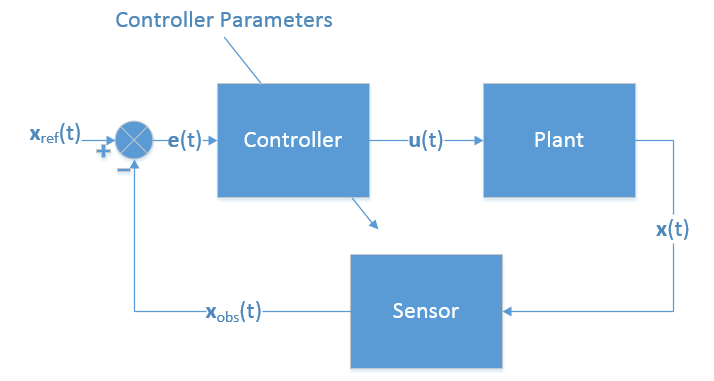
\includegraphics[width=80mm]{Controller.PNG}
\caption{Generic Controller}
\label{fig:Control}
\end{figure} 

As we can see, the controller is given the measured error vector $\mathbf{e(t)} = \mathbf{x_{ref}(t)} - \mathbf{x_{obs}(t)}$ between the desired states and observer states. It provides control inputs via the vector $\mathbf{u(t)}$ to the plant (vehicle). The plant's states $\mathbf{x(t)}$ are measured by the sensor, in our case the localization system, and fed back to the controller. The control inputs are based off of the tracked error and the previous inputs, so $\mathbf{u(t)} = \mathbf{f_{c}(e(t), u(t))}$.

As already mentioned, this architecture allows for the modification of the parameters of the controller. A controller's parameters are values that modify how the output signal $\mathbf{u(t)}$ will depend on the tracked error and the previous inputs. In essence, they define the control function, $\mathbf{f_{c}}$. Control parameters differ depending on the type of controller being used. The following subsection will provide an example of a controller and the description of its specific parameters. In any case, in this architecture these parameters are learned offline in the learning environment through the use of a model and a learning algorithm, after which the controller is brought online to control an actual vehicle.

\subsection{Model Predictive Control}

In this subsection, an MPC will be explored. An MPC may be applied to a Multi-Input Multi-Output (MIMO) system. This kind of controller produces a set of control inputs over finite prediction horizon $p$. It uses a discrete model of the system to describe the evolution of the states over this prediction horizon. To obtain a discrete linear model, the continuous model from Section \ref{sec:VehicleModel} needs to be discretized. MPC works by taking the tracking error and a generic control input vector, $\mathbf{u(t)}$, and constructing an objective function. It then minimizes this objective function with respect the the control input $\mathbf{u(t)}$. The $\mathbf{u(t)}$ value that corresponds to the global minimum of the objective function is used as the control input. The objective function is built as follows: $$J(\mathbf{e(t)}, \mathbf{u(t)}) = \sum_{i=0}^{p}(\mathbf{e(i)}^{T}Q\mathbf{e(i)}+\mathbf{u(i)}^TR\mathbf{u(i)})$$

In the function above, the limit of the summation $p$ represents the prediction horizon, or how many timesteps into the future the controller is projecting. The control output vector can be written as: $$\mathbf{u(t)} = \underset{\mathbf{u(t)}}{\mathrm{argmin}} \; J(\mathbf{e(t)}, \mathbf{u(t)})$$

The parameters of this controller are the diagonal elements of the symmetric matrices $Q$ and $R$ and the prediction horizon $p$. If we want to simplify the tuning of the controller, we can choose a constant value for the prediction horizon and only tune the matrices $Q$ and $R$. The $Q$ and $R$ matrices are usually diagonal matrices with only positive numbers to ensure that they are positive definite matrices. The diagonal entries $Q$ matrix represents the weights assigned to the different elements in the error vector. The higher the weight, the more costly that aspect of the tracking error is, and therefore the more the controller will seek to minimize that error. It is important that the relative weights of the different elements in the error vector reflect our intention, so that the controller is focusing on the most relevant aspects of the problem. The diagonal entries in the $R$ matrix represent the weights assigned to the different elements of the control vector. These weights should reflect the relative cost of responding to different control inputs, so that the more costly inputs have higher weights and are therefore less used. For example, if turning is very costly, and angular velocity is one of the inputs, the weight corresponding to angular velocity should be high to represent that it is not desirable to turn.

\section{Reinforcement Learning} \label{RLFA}

Machine learning is a technique whereby computers are taught to perform certain actions without being explicitly programmed to do so. One learning technique that has been applied to control system design is known as RL. 

\subsection{Overview}

RL is a learning paradigm whereby the agent takes actions in an environment in order to maximize the reward. This type of learning allows the agent to automatically determine the ideal behaviour within a specific context (the environment). In the case of the presented architecture, the agent is the controller and the environment is the vehicle model. The learning algorithm monitors the environment and the  results of the actions taken by the agent, and modifies the agent by reinforcing positive results and penalizing negative results as observed in the environment. Essentially, if the control signals being sent to the vehicle model result in performance that is considered desirable, then the current parameters of the controller are reinforced. A high level illustration of this architecture can be seen in Fig. \ref{fig:RL}. A more detailed, low level architecture can be seen in Fig. \ref{fig:Learn}, which will be presented in Section \ref{sec:SimulLearn}.

\begin{figure}[tb]
\centering
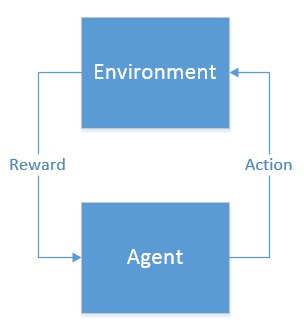
\includegraphics[width=80mm]{RL.PNG}
\caption{Reinforcement Learning}
\label{fig:RL}
\end{figure} 

\subsection{Learning Automata}

LA is one learning technique that has been previously applied to controller design. When the number of actions that the agent can take in the environment is finite, the technique is referred to as Finite Action-set Learning Automata (FALA). A detailed explanation of this can be found in~\cite{Barros-2015}. The timestep $n$ is used to denote one learning trial. The classical FALA problem can be described by the following quadruple: $$ \Gamma=(\mathcal{A}, r(n), \tau, \mathbf{p(n)})$$  

In the formulation above, 

\begin{itemize}
    \item $\mathcal{A} = \{\alpha_{1}, \alpha_{2},...,\alpha_{N_{r}}\}$ is the set of all possible actions, known as the action set
    \item $r(n)$ is the reinforcement function that specifies rewards after executing an action from the action set
    \item $\tau$ is the algorithm that is used to update the action probabilities at time $n+1$
    \item $\mathbf{p(n)} = [p_{1}(n), p_{2}(n),...,p_{N_{r}}(n)]$ is the vector that holds the probabilities that correspond to an action being taken at a given time, so $p_{i}(n)$ corresponds to the probability that action $\alpha_{i}$ will be taken at time $n$
\end{itemize}

The algorithm that updates the probability vector $\mathbf{p(n)}$, is usually formulated as follows: $$\mathbf{p(n+1)}=\tau(\mathbf{p(n)}, \alpha(n), r(n))$$

In the formulation above, $\mathbf{p(n+1)}$ represents the updated probability vector, which depends on $\alpha(n)$ (the action chosen at timestep $n$), $r(n)$, and $\mathbf{p(n)}$, which is a random process who's evolution is governed by the algorithm. When there is more than one FALA, we get a game of FALA~\cite{Narendra-1989,thathachar:2004}. In this case, we get a list of the different $\Gamma s$ that represent each individual FALA: $\mathbf{\Gamma} = (\Gamma^{1}, \Gamma^{2}, ... \Gamma^{N_{a}})$. This is important because the tuning of each controller parameter is a FALA problem, and since almost all controllers have multiple parameters, there will almost always be a game of FALA used to tune a controller, instead of just a single FALA.

\section{Architecture Implementation} \label{sec:SimulLearn}

This section will detail our specific implementation of the architecture. An MPC was designed using a game of FALA to control a differential drive robot, the Turtlebot as seen in Fig. \ref{fig:Turtle}.

\begin{figure}[tb]
\centering
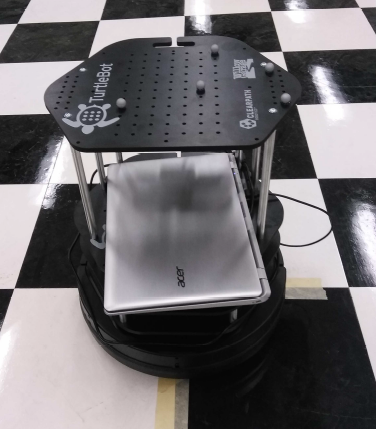
\includegraphics[width=80mm]{Turtle.PNG}
\caption{Turtlebot}
\label{fig:Turtle}
\end{figure} 

 We have seen the illustration of the architecture in Fig. \ref{fig:Arch}. Fig. \ref{fig:Impl} shows the implementation used in this experiment. The remainder of this section will describe each component in more detail.
 
\begin{figure}[tb]
\centering
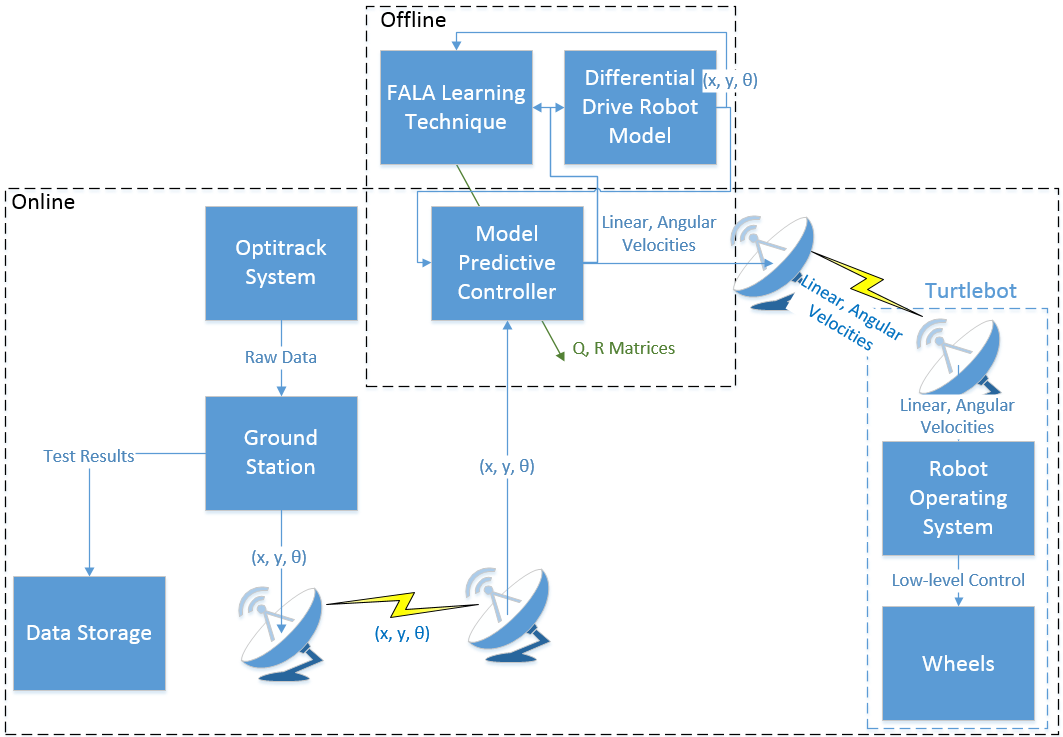
\includegraphics[width=80mm]{Impl.PNG}
\caption{Illustration of Our Implementation of the Architecture}
\label{fig:Impl}
\end{figure} 

\subsection{Optitrack System}
The localization system used for our implementation is the Optitrack System. This system uses 24 cameras arranged in a pattern around a floor space to track distinct patterns of reflectors. This system connects to the ground station via a Universal Serial Bus connection in order to feed the measurement data in for processing. 
To track the robot, the system was first calibrated. Calibration determines the position of each camera relative to the other cameras and the floor (ground plane). The result of this calibration is that the cameras are able to provide the position and orientation of any object relative to the centre of the ground plane established during the calibration phase.

Once the system was calibrated, a unique pattern of reflectors was glued on top of the robot. The pattern had to be unique to ensure that the system did not confuse the robot with any other object that was being tracked. The reflectors can be seen on top of the Turtlebot in Fig. \ref{fig:Turtle}.

\subsection{Ground Station}
The ground station is a computer that reads data from the cameras, transform sit, and then sends the position information to the controller. It also saves the data so that the controller may be validated. The ground station runs Motive, a software published by Optitrack, and a Quanser tool called Quarc to read the cameras and transform the measurement data into position and orientation information. The required information is then recorded into a file so that the performance of the controller may be validated later on, and is also sent to the controller so that it may generate control commands for the robot. The commands were sent via UDP.

\subsection{Model Predictive Controller}
The controller used is an MPC, which has already been described in Section \ref{sec:MPCForm}. It is important to note is that the controller needs a linear discrete model of the robot. In order to linearize and discretize the model of the differential drive robot described in Section \ref{sec:VehicleModel}, a linearization technique known as feedback linearization was used~\cite{he:2005}. A change of variable was done so that now $\gamma_{1} = x$, $\gamma_{2} = y$, $\gamma_{3} = \dot{x}$, $\gamma_{4} = \dot{y}$, and $\delta t$ is the timestep of the discretized model. The resulting equation is: 

\begin{multline*}
\begin{bmatrix}
\gamma_{1}(k+1) \\
\gamma_{2}(k+1) \\
\gamma_{3}(k+1) \\
\gamma_{4}(k+1) 
\end{bmatrix}
=
\begin{bmatrix}
1&0&\delta t&0\\
0&1&0&\delta t\\
0&0&1&0\\
0&0&0&1
\end{bmatrix}
\begin{bmatrix}
\gamma_{1}(k) \\
\gamma_{2}(k) \\
\gamma_{3}(k) \\
\gamma_{4}(k) 
\end{bmatrix}\\
+
\frac{1}{2}
\begin{bmatrix}
\delta t^2&0\\
0&\delta t^2\\
2\delta t&0\\
0&2\delta t
\end{bmatrix}
\begin{bmatrix}
u_{1}(k)\\
u_{2}(k)
\end{bmatrix}
\end{multline*}

The equation above is the state-space model used to represent the vehicle in the controller. The control commands, $u_{1}$ and $u_{2}$ are the accelerations in $x$ and $y$ respectively. Due to the linearization method used, it is only valid for $v \neq 0$. The control commands, $u_{1}$ and $u_{2}$ are translated to linear and angular velocities before being sent to the robot via UDP.

\subsection{Offline Learning Environment}
The previous subsections have discussed the online components of the system. These are used once the controller has been tuned. Before being brought online, the controller is tuned offline in the learning environment. The learning environment uses the vehicle model from Section \ref{sec:VehicleModel} to simulate the behaviour of the vehicle. The learning technique, a game of FALA, is used to observe the environment and modify the controller parameters. The parameters are the diagonal elements of the Q and R matrices, and are modified until the algorithm converges on parameters that achieve the desired behaviour in the model. Fig. \ref{fig:Learn} shows exactly how the learning was implemented. This is a more detailed breakdown of the architecture seen in Fig. \ref{fig:Arch} in the "Offline" box.

\begin{figure}[tb]
\centering
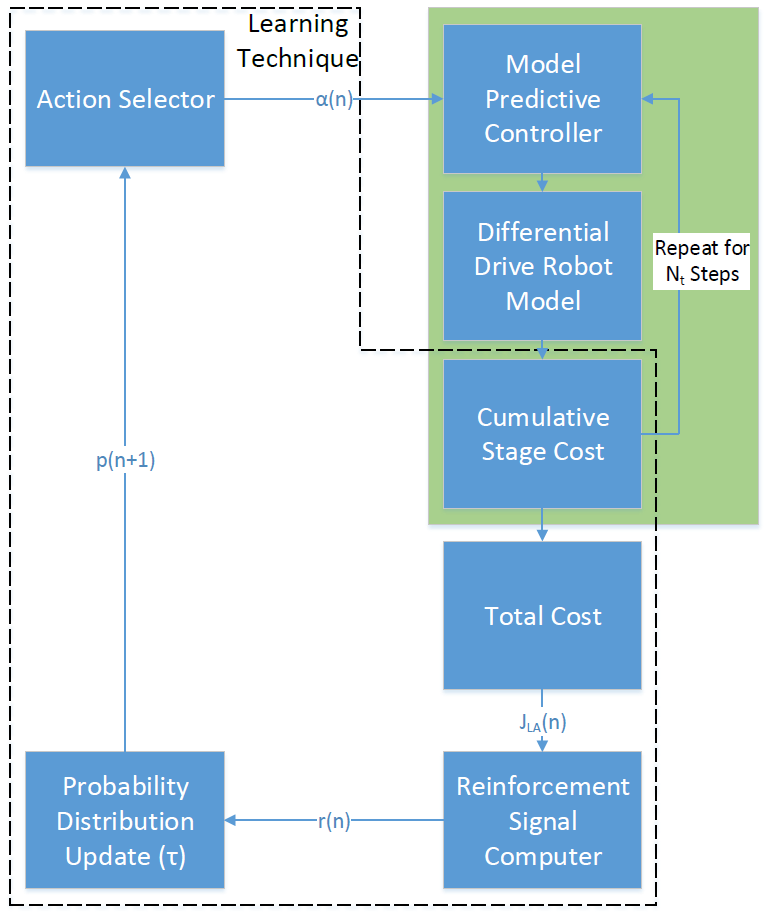
\includegraphics[width=80mm]{Learn.PNG}
\caption{Detailed Learning Architecture}
\label{fig:Learn}
\end{figure} 

For each set of parameters, we run a simulation for $N_{t}$ steps, and calculate the total tracking error $e(t)$ by adding up all the euclidean errors between the model's behaviour (location) and the desired location. This total cost is calculated using the error function: $$J_{LA}(n) = \sum_{t=1}^{N_{t}}[k_{p}(e(t))^2+k_{d}\frac{d}{dt}e(t)]$$ and is a scalar value that represents the error. The constants $k_{p}$ and $k_{d}$ define the relative importance of the different error components. This then feeds into the reinforcement signal computer, which calculates the reinforcement signal 
$$r(n) = R_{b}\min(\max(0, \frac{J_{LA,med}-J_{LA}(n)}{J_{LA}(n)-J_{LA,min}}), 1)$$ 
based off of the error. $J_{LA,med}$ represents the mean error over the iterations, $J_{LA,min}$ represents the minimum error, and $R_{b}$ is the upper limit of a term used to accelerate the training. Lastly, this is fed into the probability distribution update function $\tau$, which updates the probability vector $$\mathbf{p^{i}(n+1)} = \frac{\mathbf{p^{i}(n)}+\lambda r(n)\mathbf{p^{i}(n)}}{|\mathbf{p^{i}(n)}+\lambda r(n)\mathbf{p^{i}(n)}|}$$ using the learning rate $\lambda$. This is the passed to the action selector, which modifies the parameters in the controller via the signal $\mathbf{\alpha(n)}$, and the steps are repeated until the best results are achieved. 

As already mentioned, the controller was tuned by having the robot follow a series of waypoints. The set of waypoints that the robot was trained on, the progression of the path, and the visualization of this environment can be seen in Fig. \ref{fig:Env}.

\begin{figure}[tb]
\centering
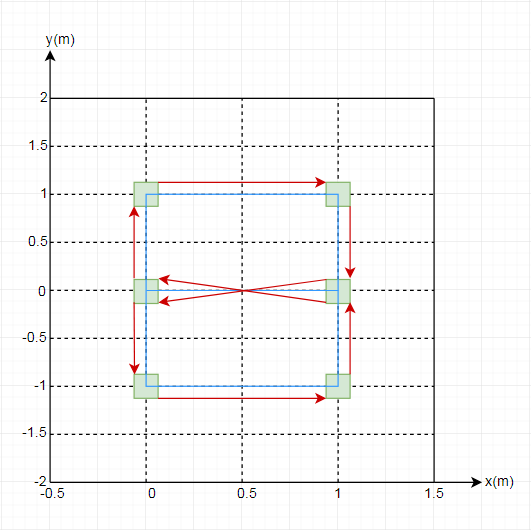
\includegraphics[width=80mm]{Env.PNG}
\caption{Waypoints Used to Tune the Controller}
\label{fig:Env}
\end{figure} 

\subsection{Turtlebot}

In our implementation of the architecture we used the Turtlebot, which is a differential drive robot controlled through a middleware framework known as the Robot Operation System (ROS). ROS allows for communication and computation distribution.

\section{Results} \label{sec:Results}

In order to verify the testing environment and to demonstrate that the learned parameters of the controller performed better than the designed ones, the robot was given a moving reference in the shape of a figure eight. The learned parameters performed measurably better than the designed parameters. Additionally, the testing environment allowed for fast and easy comparison of the parameters. Fig. \ref{fig:Path} shows the reference, the path as performed with the designed parameters, and the path as performed with the learned parameters.

\begin{figure}[tb]
\centering
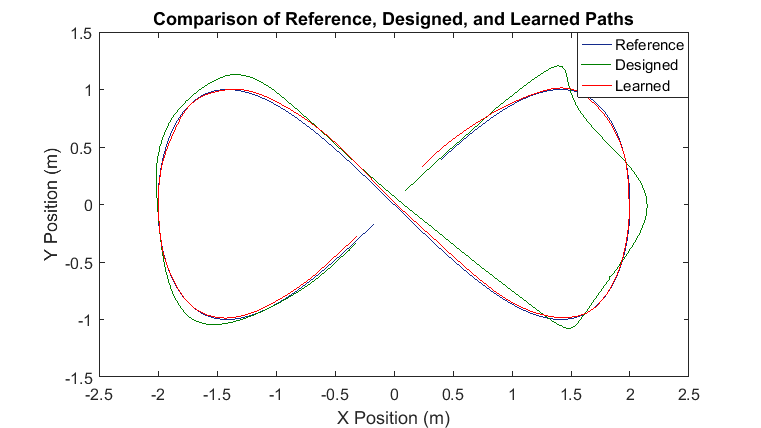
\includegraphics[width=80mm]{Path.png}
\caption{Illustration of the Paths Taken by the Designed and Learned Parameters}
\label{fig:Path}
\end{figure} 

While it may appear evident from the illustration in Fig. \ref{fig:path} that the learned parameters perform better than the designed parameters, it is important to demonstrate this mathematically. Ten runs were done for each type of tuning. Then, the Mean Square Error was calculated for each run. Each type of tuning now had a sample set of ten Mean Square Error values. In order to show that the two sample sets were not drawn from the same distribution a Student's t-test was done. The null hypothesis was rejected with $p<0.01$, which meant that the two sample sets were demonstrably different. Lastly, box plots for the two sample sets were made to visualize the difference between the two. These box plots can be seen in Fig. \ref{fig:Results}.

\begin{figure}[tb]
\centering
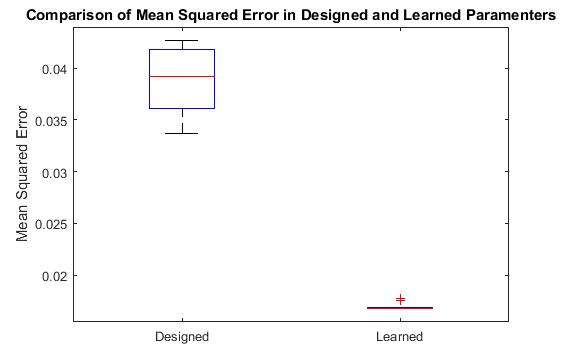
\includegraphics[width=80mm]{Results.png}
\caption{Comparison of Designed and Learned Parameters}
\label{fig:Results}
\end{figure} 

As we can see from the plot in Fig. \ref{fig:Results}, the learned parameters did indeed perform much better than the designed parameters. This demonstrates the efficacy of FALA as an MPC weight tuning technique. Furthermore, all of the data necessary to compare the two controllers was readily available due to the architecture providing constant position information about the robot, allowing us to see how well each controller performed tracking the moving figure eight reference. This demonstrates that the testing architecture presented in this paper is a good way to compare different controllers.

\section{Conclusion} \label{sec:conc}

To conclude, this paper presents an architecture that provides a way for fast and effective comparison between different controllers. The architecture relies on a localization system combined with a ground station to provide feedback to a generic controller which has been tuned offline using a machine learning technique. The controller then generates commands which are fed to a vehicle computer that turns them into low level control signals for the actuators on the vehicle. This architecture was implemented by tuning an MPC through FALA to control a differential drive robot. Two controllers were easily compared through the data obtained from the testing architecture. This demonstrated the efficacy of the testing architecture presented in this paper. This architecture may be used to test any controller, tuned with any machine learning technique, and controlling any vehicle.

\balance

\bibliographystyle{IEEEtran}
\bibliography{journal}





% trigger a \newpage just before the given reference
% number - used to balance the columns on the last page
% adjust value as needed - may need to be readjusted if
% the document is modified later
%\IEEEtriggeratref{8}
% The "triggered" command can be changed if desired:
%\IEEEtriggercmd{\enlargethispage{-5in}}

% references section

% can use a bibliography generated by BibTeX as a .bbl file
% BibTeX documentation can be easily obtained at:
% http://mirror.ctan.org/biblio/bibtex/contrib/doc/
% The IEEEtran BibTeX style support page is at:
% http://www.michaelshell.org/tex/ieeetran/bibtex/
%\bibliographystyle{IEEEtran}
% argument is your BibTeX string definitions and bibliography database(s)
%\bibliography{IEEEabrv,../bib/paper}
%
% <OR> manually copy in the resultant .bbl file
% set second argument of \begin to the number of references
% (used to reserve space for the reference number labels box)




% that's all folks
\end{document}


